A detailed study of the impact of the phenomenon of interference between the signal process $gg \rightarrow H \rightarrow \gamma\gamma$ and its irreducible background process $gg \rightarrow \gamma\gamma$ has been made in \cite{ATL-PHYS-PUB-2016-009}. It will be summarised below.

All the results from \cite{ATL-PHYS-PUB-2016-009} have been made with simulated data for the $\sqrt{s} = 8$ \UTeV dataset. A full-fledged extrapolation to higher centre of mass energies remains to be done. However, the two processes that interfere together, are induced by the same initial state and are at a similar mass scale. All the results are based on a difference between results made with simulated data where the interference have been implemented in the simulation, and simulated data where it is not. In the following, we will therefore consider that any increase of the cross-section with respect to $\sqrt{s}$ will cancel out in the difference.

The main goal of \cite{ATL-PHYS-PUB-2016-009} was a robust estimate of the mass shift induced by the interference between $gg \rightarrow H \rightarrow \gamma\gamma$ and its irreducible background process $gg \rightarrow \gamma\gamma$ within the Standard Model (SM). This was achieved by using the Monte-Carlo generator Sherpa 2.0, that provides a specific plug-in allowing to generate datasets of weighted events, corresponding either to the the signal term ($gg \rightarrow H \rightarrow \gamma\gamma$ amplitude), the irreducible gluon-induced background term ($gg \rightarrow \gamma\gamma$ amplitude), their interference term or a any combination of these processes. The Feynman diagram describing the different processes involved are given in fig. \ref{fig:intef_diags}. 

\begin{figure}
    \centering
    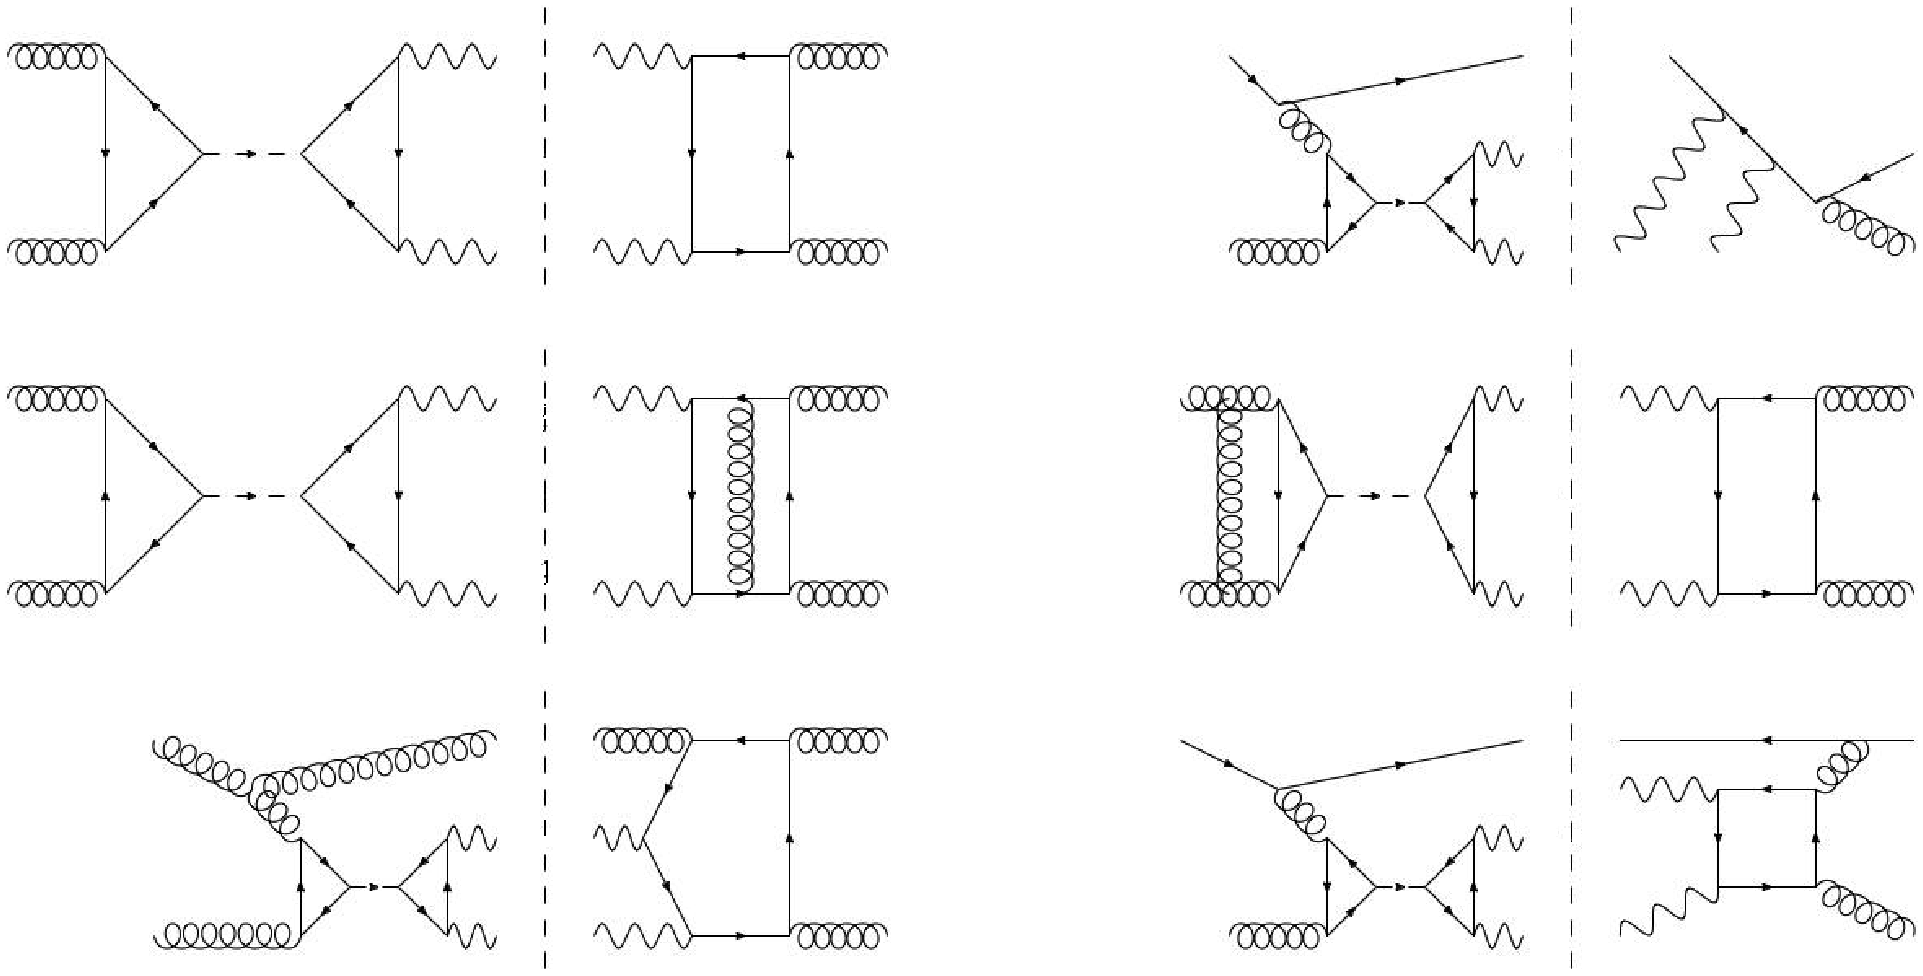
\includegraphics[width=0.85\textwidth]{\main/section5/plots/intef_diags.png}
    \caption{Feynman diagrams describing the various processes involved in the phenomenon of interferences between $H\rightarrow\gamma\gamma$ and its background,}
    \label{fig:intef_diags}
\end{figure}

It was the first time that Sherpa 2.0 was used in an analysis, and in particular the only time its interference module has been used. The distribution of the di-photon pair transverse momentum ($P_T^{\gamma\gamma}$) has been studied in detailed, as it is a preliminary requirement to be able to recast the mass analysis described in \cite{Aad:2014aba}. To get the best match of the $P_T^{\gamma\gamma}$ distribution between this simulation and the state of the art estimates, Sherpa 2.0 had to be tuned. This was done by varying the parameter $CSS\_IS\_AS\_FAC$ that controls the scale at which the parameter $\alpha_S$ is evaluated during parton shower evolution for the initial state. Simulated data samples were generated at several values of this parameter and compared to prediction for the Higgs boson transverse momentum from HRes2.0. The value of $CSS\_IS\_AS\_FAC$ for which both predictions were agreeing the best has been kept for the simulations used for the final result. The distributions of $P_T^{\gamma\gamma}$ obtained for a simulation of the background has been compared between ResBos and Sherpa2.0 for the best value of $CSS\_IS\_AS\_FAC$. They were found to be in reasonable agreement.

Then large samples of weighted signal (S) and interference (I) events were simulated. The background component was determined using a data-driven method (B). The background functions described in \cite{Aad:2014aba} were re-used, and they were fitted to the $\sqrt{s} = 8$ \UTeV dataset. This allowed to construct two varieties of simulated $m_{\gamma\gamma}$ templates, one that was made of $S+B$ and the other of $S+B+I$. These samples were then folded by the energy resolution and photon efficiencies used in \cite{Aad:2014aba} to mimic the detector simulation. The di-photon mass distributions induced by these different terms can be found in fig. \ref{fig:interfer_lineshape}. The Higgs boson mass ($m_H$) is measured separately on both templates, giving the values of $m_H$ including the impact of interference ($m_H^{S+B+I}$), and without ($m_H^{S+B}$). Then the impact of the interference term itself on $m_H$ is determined as \begin{equation}
    \Delta m_H = m_H^{S+B+I}-m_H^{S+B}.
\end{equation}

\begin{figure}
    \centering
    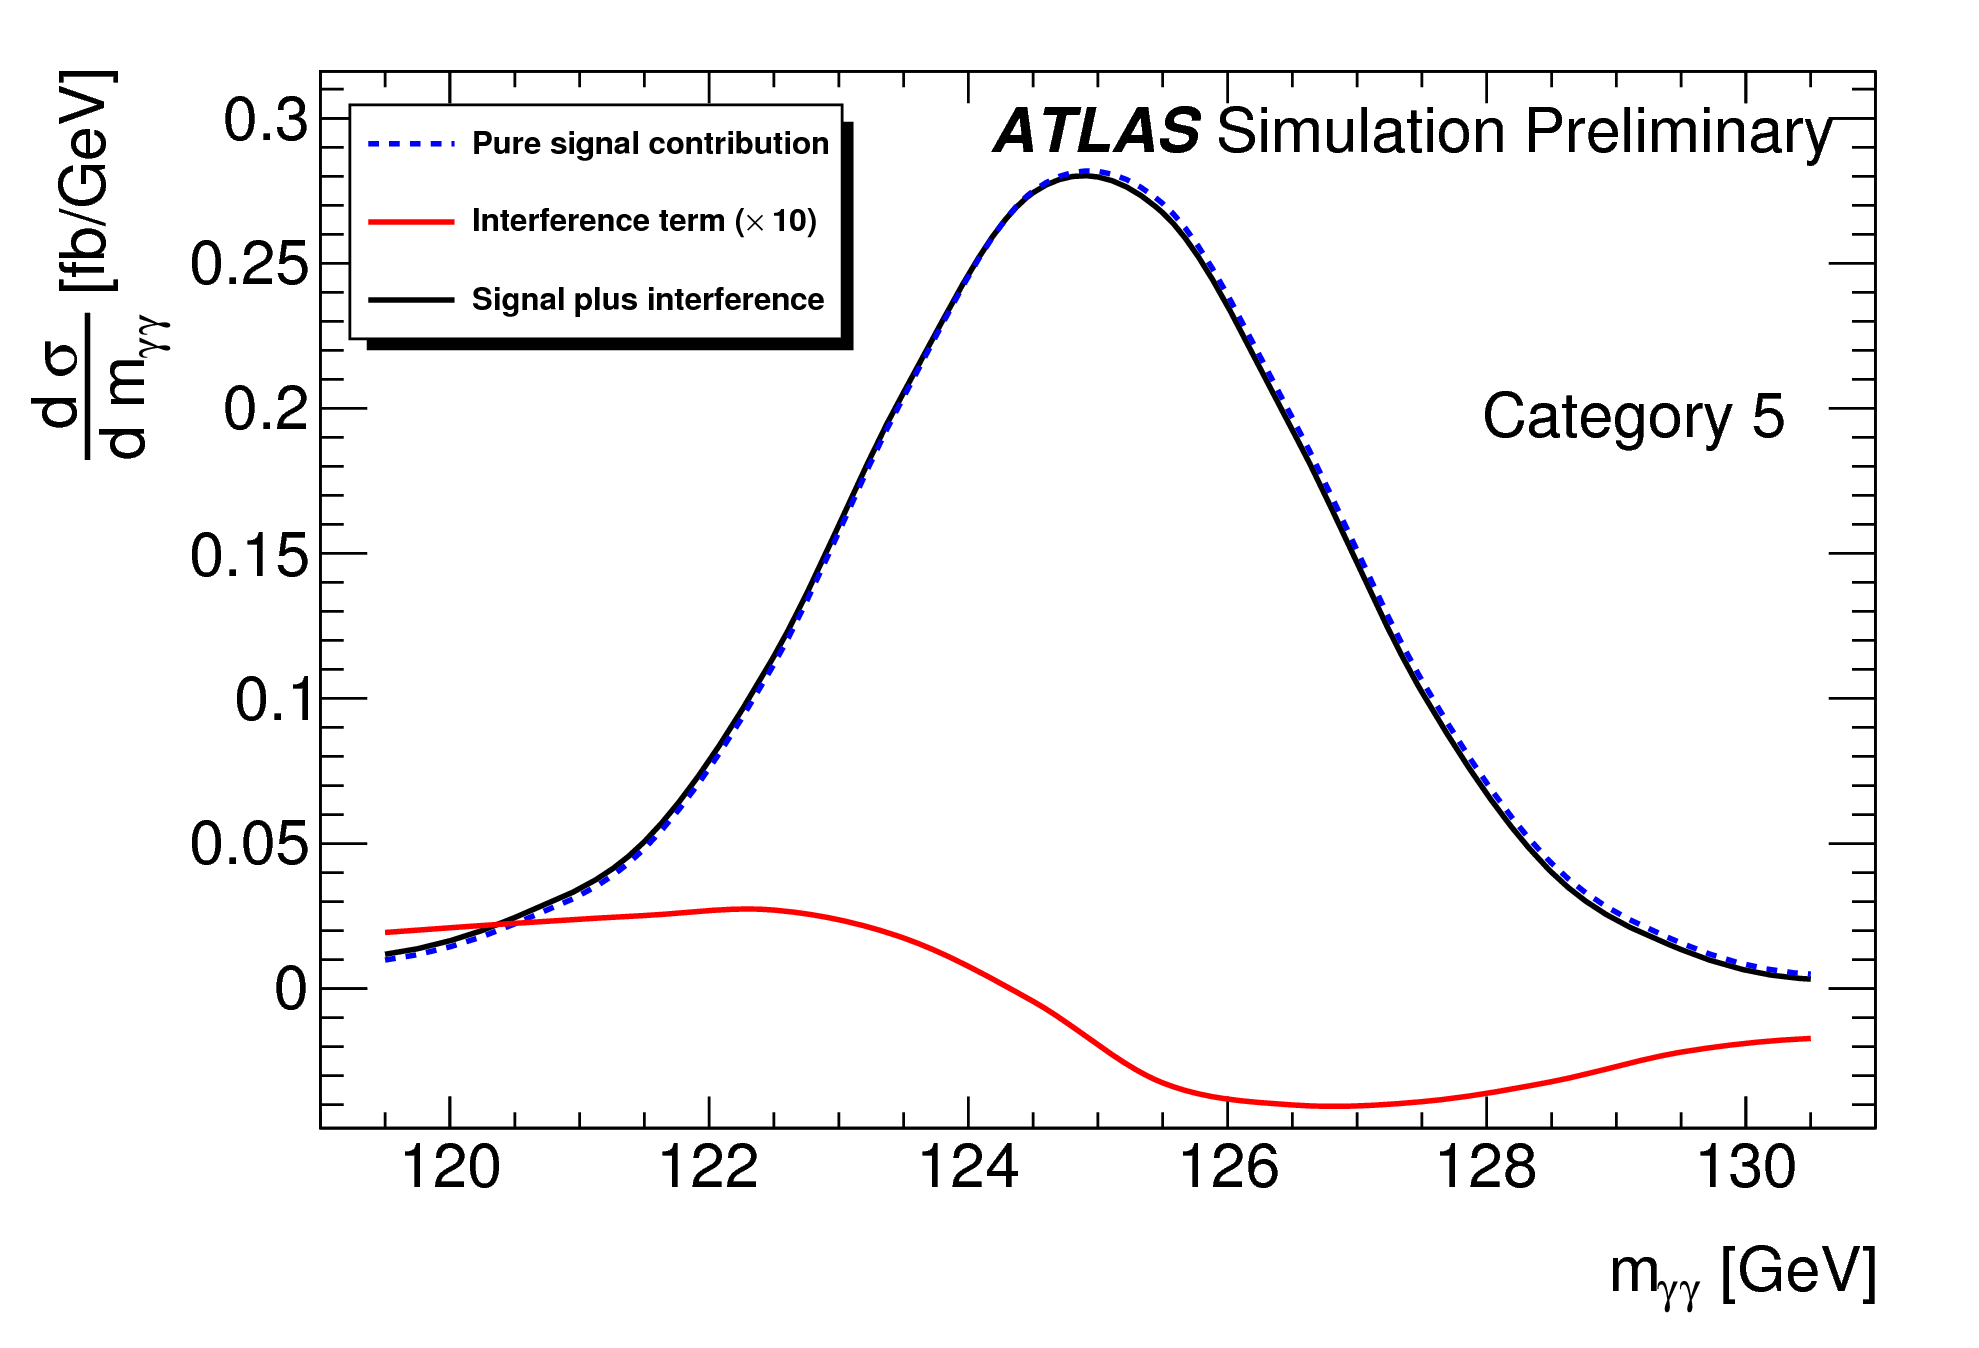
\includegraphics[width=0.6\textwidth]{\main/section5/plots/interfer_lineshape.png}
    \caption{Di-photon invariant mass distribution for signal and interference terms.}
    \label{fig:interfer_lineshape}
\end{figure}

Several uncertainties have been considered. First a non-closure of 3 \UMeV has been observed while measuring $m_H^{S+B}$ from the S+B simulated sample, and is propagated as an experimental uncertainty. The only other experimental uncertainty stems from the choice of background function, and has been estimated at 3 \UMeV by trying different background functions.

For theoretical uncertainties we considered both scale variations as well as K-factor variations, as we will describe now.
The renormalisation  and factorisation scales were varied by a factor of 2, between $\frac{1}{2}~m_{\gamma\gamma}$ and $2~m_{\gamma\gamma}$ (the nominal value is $m_{\gamma\gamma}$). The resummation scale itself was varied between $\frac{1}{4}~m_{\gamma\gamma}$ and $2~m_{\gamma\gamma}$. Samples were re-generated at these different values of the scales for S and I, and the value of $\Delta m_H$ was re-evaluated. This gave a small uncertainty of $\pm 4$ \UMeV, which can be explained by the migration of events between transverse momentum categories that leads to a cancellation of these variations in the difference $\Delta m_H$.

The signal K-factor ($k_S = \dfrac{NNLO}{NLO}$) has been varied by 0.1, between $k_S = 1.35$ and $k_S = 1.55$. The background K-factor $k_B$ is not known, and it was decided to vary it between 1 and $k_S$. The recipe gave an uncertainty of $\pm 7$ \UMeV, which is the dominant uncertainty. Constraining $k_B$ could lead to a huge improvement, but it requires to separate the component $gg \rightarrow \gamma\gamma$ from the inclusive $pp \rightarrow \gamma\gamma$ production. This is expected to be complicated but might be achieved by the study of angular distributions in $pp \rightarrow \gamma\gamma+jets$.

This study conducted to the following estimate of the Higgs boson mass shift induced by the interference process within the Standard Model :

\begin{equation}
    \Delta m_H = -35 \pm 8 {\rm{(theory)}} \pm 4 {\rm{(experimental) \UMeV}}.
\end{equation}

The mass shift was also determined for larger widths, in the specific scenario where the width is modified but the expected number of events around the di-photon peak (S+I), is not. The mass shift was determined to be $\Delta m_H = -313\pm 72$ \UMeV for $\Gamma_H = 300$ \UMeV and $\Delta m_H = -453 \pm 106$ \UMeV for $\Gamma_H = 600$ \UMeV. By the end of HL-LHC such deviations could be probed by comparing the mass measured in the high-precision $H\rightarrow 4l$ channel and the one measured in $H\rightarrow\gamma\gamma$. The following difference :
\begin{equation}
    \delta m_H^{4l-\gamma\gamma} = m_H^{4l} - m_H^{\gamma\gamma}
\end{equation}
will be largely dominated by the systematic uncertainty on $m_H^{\gamma\gamma}$. Assuming it is at the same level than the one of Run 2 \cite{Aaboud:2018wps}, it would lead to an uncertainty on the measured $\delta m_H^{4l-\gamma\gamma}$ of 290 \UMeV, hence a shift of 580 \UMeV could be excluded at 95\% C.L. Also assuming that $\delta m_H^{4l-\gamma\gamma}$ scales linearly with the Higgs boson width, it would allow in this naive model, to set upper limits on the Higgs boson width at $\Gamma_H < 1$ \UGeV at 95\% C.L.

This is only using the difference between the Higgs boson mass measured in its 4 leptons decay channel and the one measured in its di-photon decay channel. Now, it is also known that the interference term will have a bigger impact in some parts of the phase space where the signal to background ratio is smaller. This is for instance the case at low $p_T^{\gamma\gamma}$, and it could be used to carry out the same inference internally in the $H\rightarrow\gamma\gamma$ channel, comparing the masses measured in two (or more) $p_T^{\gamma\gamma}$ bins. A full-fledged prospect study of this analysis remains to be done, as the only attempt carried out so far \cite{ATL-PHYS-PUB-2013-014} suffered from large mis-modellings of the kinematic distributions and of the cross-sections. The success of such an analysis will rely on very precise predictions for the kinematic distributions, which is not yet available. This will require the development of new higher-order calculations and resummed predictions, and could be helped by the development of new Monte-Carlo tools using better showering algorithms.